\documentclass{leptc}
\usepackage{tikz}
\usepackage{moreverb}
\usetikzlibrary{shapes,shadows,calc}
\usetikzlibrary{arrows,decorations.markings}
\begin{document}
\chap{乌云漏洞整理}
整理者:\href{mailto:lxy_September@outlook.com}{李欣宜} \\
文档源码地址:\url{https://github.com/Lixinyi-DUT/Project-Wuhu}\\
整理自\href{http://www.wooyun.org/}{乌云漏洞平台}\\
%\tableofcontents
\chap{第一周}
\begin{center}
	\com{2015/6/29-2015/7/3}
\end{center} 

\chaps{6/29 中国移动某IP依旧可心脏滴血(可泄露用户服务密码等信息)}
\begin{center}
	\url{http://www.wooyun.org/bugs/wooyun-2015-0122764}
\end{center}
\enl{提交时间} 2015/6/25 \\
\enl{确认时间} 2015/6/29 \\
\enl{漏洞hash} 183e27ad5344f8c03dfa1cb97a16be59 \\
\enl{漏洞类型} 系统/服务补丁不及时 \\
\enl{简要描述} 中国移动某IP存在OpenSSL漏洞-(可泄露用户服务密码等信息)\\
\ent[ heartbleed bug]{心脏出血漏洞}是出现在加密库\ent{OpenSSL 1.0.1}\com{实现SSL与TLS协议}上的程序错误,可允许攻击者读取服务器的内存信息,客户端和服务器都可能因为这个漏洞受到攻击。该漏洞得名于\ent[\B Transport \B Layer \B Security]{TLS协议}和于\ent[\B Dategram \B Transport \B Layer \B Security]{DTLS协议}中已成为标准的机制\ent[heartbeat extension]{心跳扩展},它提供了一种测试和保持安全通信链路的方式,而无需每次都重新协商连接,但这种扩展没有进对输入行有效验证,即\ent[bounds check]{边界检查},导致了\ent[buffer over-read]{缓冲区过读},因此引发信息泄露。受影响的OpenSSL版本为1.0.1至1.0.1f(含),而较早的版本和较新的版本均没有受到影响。\\
\enl{漏洞影响} 约有17\%通过认证机构认证的互联网安全网络服务器被认为容易受到攻击,导致服务器私钥和用户会话cookie及密码被盗。\\
\enl{补救措施} OpenSSL版本1.0.1g增加了一些边界检查,以防止过度读取缓冲。例如,已添加了下列测试,以丢弃将引发心脏出血漏洞的心跳请求,阻止回复继续构建:\\
	\verb|if (1 + 2 + payload + 16 > s->s3->rrec.length) return 0;|\\
存在缺陷的服务器应及时升级系统和服务补丁,疑似受到攻击的这些应用服务的用户也被建议及时更换密码等信息,并获取系统的更新。一些网站推出了测试,检测给定的网站上是否存在心脏出血漏洞,比如\href{http://heartbleed.criticalwatch.com/}{Critical Watch免费在线心脏出血测试器}, \href{https://blog.lookout.com/blog/2014/04/09/heartbleed-detector/}{Lookout Mobile Security心脏出血探测器}\com{一个用于Android设备的应用程序,可确定设备使用的OpenSSL版本,并指出是否启用了有缺陷的心跳特性}和\href{https://www.ssllabs.com/ssltest/}{Qualys}\com{SSL实验室的SSL服务器测试,不仅能查找心脏出血漏洞,还能找到其他位于SSL/TLS实现中的错误}等。\\

\chaps{6/30 TCL某站后台弱口令导致整站webshell部分VIP会员信息泄露}
\begin{center}
	\url{http://www.wooyun.org/bugs/wooyun-2010-0123296}
\end{center}
\enl{提交时间} 2015/6/28\\
\enl{漏洞类型} 后台弱口令 \\
\enl{漏洞细节} 图片见该漏洞的\href{http://www.wooyun.org/bugs/wooyun-2010-0123296}{报告地址},这里不再给出
\begin{enumerate}
	\item 进入网站\url{http://tvp.multimedia.tcl.com/sysadmin/login.aspx}
	\item
	使用弱口令 \verb|admin/toprand| 登录
	\item
	修改上传设置,在图片类型中增加asp和aspx类型
	\item
	将\href{http://tvp.multimedia.tcl.com/UploadFiles/Images/2015/6/20150628152911.aspx}{测试文件}上传Shell,可以得到服务器的安全信息
	\item
	删除后发现VIP用户信息泄露
\end{enumerate}

\enl{漏洞简述} \ent[weak password]{弱口令}通常是指容易被人猜测或者被破解工具破解的口令,一般仅包含简单的数字和字母。可以通过\ent[weak password dictionary]{弱口令字典}以一定概率扫描获得。口令强度可以用微软提供的\href{http://www.microsoft.com/zh-cn/security/pc-security/password-checker.aspx}{密码检查器}进行评估。\\
\enl{补救措施} 修改弱口令,升级后台系统。\\

\chaps{7/1 华融证劵某站补丁不及时导致getshell(可内网渗透)}
\begin{center}
	\url{http://www.wooyun.org/bugs/wooyun-2015-0111837}
\end{center}
\enl{提交时间} 2015/5/12 \\
\enl{公开时间} 2015/6/29 \\
\enl{漏洞类型} 成功的入侵事件 \\
\enl{漏洞细节} 站点:\url{http://oa.hrsec.com.cn/login/Login.jsp?logintype=1} \\
使用泛微oa找到弱口令进入,上传测试文件后,直接getshell,获得了root权限。\\
\enl{漏洞简述} 泛微oa系统存在着很大的缺陷,使用定制泛微oa的厂家的信息安全也因此受到了很大的威胁。不及时打补丁的使用厂家尤甚,\ent{SQL注入}和\ent{弱口令}都可能使没有合法权限的入侵者进入系统后台,由于\ent{任意文件上传}威胁的存在,攻击者可以上传制作好的测试脚本获得root权限。\\
\ent{WebShell}是以asp、php、jsp或者cgi等网页文件形式存在的一种命令执行环境,也可以将其称做为一种网页后门。\\
入侵者通常会将这些asp或php后门文件与网站服务器WEB目录下正常的网页文件混在一起,然后就可以使用浏览器来访问这些asp或者php后门,得到一个命令执行环境,以达到控制网站服务器的目的,这就是\ent{WebShell攻击}。\\
这种攻击也可以通过\href{https://github.com/cfc4n/pecker}{Pecker Scanner工具}进行检测。\\
\enl{补救措施} 及时更新系统补丁,遵循\ent{最低权限原则}。\\

\chaps{7/2 趣分期撞库漏洞(成功98个)}
\begin{center}
	\url{http://www.wooyun.org/bugs/wooyun-2015-0114565}
\end{center}
\enl{提交时间} 2015/5/18 \\
\enl{公开时间} 2015/7/2 \\
\enl{漏洞类型} 设计缺陷/逻辑错误 \\
\enl{漏洞细节} 撞库接口:\url{http://www.qufenqi.com/login} 频繁测试受到限制时换IP列表继续测试\\
\enl{漏洞简述} \ent{拖库攻击}指入侵有价值的网络站点,把注册用户的资料数据库全部盗走的行为。取得大量的用户数据之后,黑客会通过一系列的技术手段和黑色产业链将有价值的用户数据变现,这通常也被称作\ent{洗库}。最后黑客将得到的数据在其它网站上进行尝试登陆,叫做\ent{撞库},因为很多用户喜欢使用统一的用户名密码。\\
为了应对这种攻击,有时企业会在登录页面加上验证码,然而识别图像验证码的脚本并不难获得,所以收效甚微。与之类似,对于IP和输入密码错误次数限制也是出于同样的考虑,但还是难以防止有针对性的恶意攻击。\\
\enl{补救措施} \N1 对于用户来说,尽量不要在不同的网站使用统一的用户名和密码,如果有使用,那么一旦发现其中某个网站的信息泄露,立即更换其他站点使用的密码。\N2 对于应用的运营商,除了增强数据库常规的安全手段,也可以从多维度入手防止撞库扫号,比如增加手机验证码验证,或者使用\ent{Flash Cookies}代替\ent{Cookies}。\\
\begin{center}
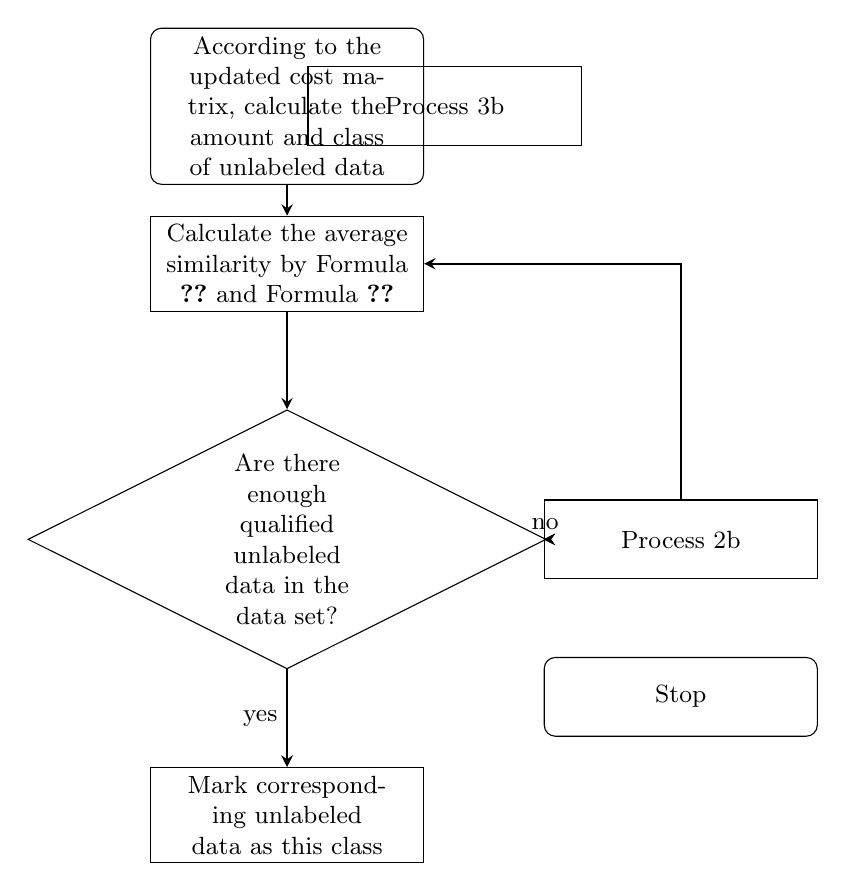
\begin{tikzpicture}[node distance = 2cm, auto]
{\small
	\tikzstyle{startstop} = [rectangle, rounded corners, minimum width=3cm, minimum height=1cm, text width=10em, text centered, draw=black]
	\tikzstyle{process} = [rectangle, minimum width=3cm, minimum height=1cm, text centered, text width=10em, draw=black]
	\tikzstyle{decision} = [diamond, aspect=2, minimum width=.5cm, minimum height=.5cm, text centered, text width=5em, draw=black]
	\tikzstyle{arrow} = [thick,->,>=stealth]

	\node (start) [startstop] {According to the updated cost matrix, calculate the amount and class of unlabeled data};
	\node (pro1) [process, below of=start] {Calculate the average similarity by Formula \ref{formula15} and Formula \ref{formula16}};
	\node (dec1) [decision, below of=pro1, yshift=-1.5cm] {Are there enough qualified unlabeled data in the data set? };
	\node (pro2a) [process, below of=dec1, yshift=-1.5cm] {Mark corresponding unlabeled data as this class};
	\node (pro2b) [process, right of=dec1, xshift=3cm] {Process 2b};
	\node (pro3b) [process, above of=pro2b, right of=pro1] {Process 3b};
	\node (stop) [startstop, below of=pro2b] {Stop};
	\draw [arrow](start) -- (pro1);
	\draw [arrow](pro1) -- (dec1);
	\draw [arrow](dec1) -- (pro2a);
	\draw [arrow](dec1) -- (pro2b);
	\draw [arrow](dec1) -- node[anchor=east] {yes} (pro2a);
	\draw [arrow](dec1) -- node[anchor=south] {no} (pro2b);
	\draw [arrow](pro2b) |- (pro1);
	}
\end{tikzpicture}
\end{center}

\label{attention}
\chaps{7/3 上海虹桥火车站Wi-Fi认证设计不当导致绕过漏洞}
\begin{center}
	\url{http://www.wooyun.org/bugs/wooyun-2015-0112807}
\end{center}
\enl{提交时间} 2015/5/8 \\
\enl{公开时间} 2015/6/26 \\
\enl{漏洞类型} 设计缺陷/逻辑错误 \\
\enl{漏洞细节} 填手机号,发送验证码之后,抓包。可以看到返回信息中直接包含了验证码。这样也就绕开了短信接收验证码然后再输入验证的过程,无法进行身份验证。\\
\enl{漏洞简述} \ent{Wi-Fi Portal认证}是开放WLAN中验证用户身份的一种方式,我校的无线网络DLUT也是使用的这种认证机制。在机场、火车站、咖啡厅等公共场所的WLAN一般应用\ent[Challenge-Response authentication]{挑战/应答认证}对接入者身份进行验证,比如短信接收验证码。这种认证中,用户填写的个人信息请求通过\ent[POST method]{POST方法}传给服务器,而这个\verb|POST|请求的数据包中就含有用户的个人信息,在Web条件下,可以通过IE或者Chrome自带的抓包工具获得,我曾经利用过这个方法写了一个\href{https://github.com/Lixinyi-DUT/WirelessHelper}{实现DLUT后台自动登录的应用},也是利用了DLUT数据包明文传输的缺陷。\\
\fig[0.7]{packet.png}\\
\enl{补救措施} 数据包中的验证码加密,或者在认证中心建立可靠的数据库管理这些验证码,而避免验证信息在数据包中传递。\\

\chap{第二周}
\begin{center}
	\com{2015/7/6-2015/7/10}
\end{center}

\chaps{7/6 联想手机VIBE UI部分版本设计缺陷绕过锁屏读所有联系人}
\begin{center}
	\url{http://www.wooyun.org/bugs/wooyun-2015-0105688}
\end{center}

\enl{提交时间} 2015/4/3 \\
\enl{公开时间} 2015/7/6 \\
\enl{漏洞类型} 设计错误/逻辑缺陷 \\
\enl{漏洞细节} \N1 机型:\texttt{A355e} \N2 \texttt{VUBE UI}的版本:\verb|A355e_S020_20141229| \N3 向测试手机拨打电话,然后这个时候往上滑动,进入自定义短信回复界面 \N4 进入短信回复界面以后,在联系人框那里随便输入一个数字,比如一般手机号开头都是1,这样就可以读到所有联系人了。\\
\enl{漏洞简述} \texttt{iOS7}也曾经出现过可以绕过锁屏的安全漏洞,而\texttt{Android}系统由于各个厂家的定制UI,对安全问题的重视程度不一,也经常存在同样的问题。\texttt{Android}应用\href{http://secretlisa.com/words-screen-lock/}{单词锁屏}也存在这个漏洞,下拉状态栏可以直接进入其他应用而绕过锁屏,强迫自己背单词不玩手机的目的也就无法达到。\\
这种漏洞存在的原因很多,在\texttt{Android 4.3}中\code{com.android.settings.ChooseLockGeneric}是负责更改系统的解锁方式的类,再解锁确认后它的成员\code{mPasswordConfirmed}被设置为\code{True},这个成员没有私有保护,从外部启动\code{ChooseLockGeneric}再设置这个参数,设定密码策略为\code{PASSWORD_QUALITY_UNSPECIFIED}\com{对密码没有要求},系统就会自动清除锁屏密码,更多其他方法可以自行查阅。\\
\enl{补救措施} \N1 把逻辑设置为自定义回复短信的时候需要输入解锁密码 \N2 学习华为的最新系统,把在通话界面实现自定义回复短信的功能用另外的模块实现,在这个模块中只有短信内容框别的什么都没有。 \N3 参考\texttt{Android}原生系统,对\code{mPasswordConfirmed}进行保护。\\

\chaps{7/7 墨迹天气可以重置任意用户密码}
\begin{center}
	\url{http://www.wooyun.org/bugs/wooyun-2015-0115443}
\end{center}
\enl{提交时间} 2015/5/22 \\
\enl{公开时间} 2015/7/6 \\
\enl{漏洞类型} 网络设计缺陷/逻辑错误 \\
\enl{漏洞细节} \N1 找回密码页面\url{http://uc.mojichina.com/findpwd/byphone#}填写手机号和验证码,点下一步 \N2 网页自动跳转到页面\url{http://uc.mojichina.com/findpwd/verifysms} \N3在同一个浏览器中再打开网页\url{http://uc.mojichina.com/findpwd/resetpwdbyphone#},就直接进入重置密码界面了,不需要短信验证码的确认。\\
\enl{漏洞简述} 这是程序设计的严重缺陷,致使边界绕过,也类似\ent[URL redirection]{URL重定向跳转}漏洞。在一个页面认证完成之前就可以通过重定向跳转到本应该完成认证后出现的页面,这是认证设计上完全可以避免的漏洞。\\

\chaps{7/8 苏宁易购服务器支持EXP密码套件可SSL FREAK攻击解密通信流量(含poc)}
\begin{center}
	\url{http://www.wooyun.org/bugs/wooyun-2015-0106650}
\end{center}
	\enl{提交时间} 2015/4/8 \\
	\enl{公开时间} 2015/7/8 \\
	\enl{漏洞类型} 默认配置不当 \\
	\enl{漏洞细节} 苏宁易购服务器因支持EXP密码套件,遭受SSL FREAK攻击,中间人可在线解密通信流量(获取到登陆凭证等敏感信息)
    \begin{itemize}
    	\item 服务器会接受\texttt{EXP-DES-CBC-SHA(SSLv3、TLSv1)}、\texttt{EXP-RC2-CBC-MD5(SSLv3、TLSv1)}、\texttt{EXP-RC4-MD5(SSLv3、TLSv1)}这三种\ent[export-grade cipher suite]{出口级密码套件}\com{EXP密码}。
    	\item 以登陆页面\url{https://passport.suning.com/ids/login}为例,\ent[man in the middle]{中间人}在受此漏洞影响的客户端(如还未打补丁的IE、Chrome、Safari、Opera on Mac OS等)访问页面时,如果有中间人发起FREAK攻击,将\texttt{client hello}消息中的密码套件改为EXP类别,那么服务器会选择使用EXP级别的密码套件进行通信,发送512bit\ent[\B Rivest-\B Shamir-\B Adleman public key]{RSA公钥}给客户端。
    	\item 客户端用这个512bit的公钥加密\ent[pre-master secret]{预主密钥},服务器收到后用私钥解密出预主密钥,两方依据此秘密信息同时计算出后续通信的密钥。
    	\item 而对于中间人来说,如果其可以分解服务器发送的512bit的公钥,那么即可计算出私钥,从而也同样可以得到预主密钥,进而算出通信的密钥,解密客户端和服务器的通信内容。 
    	\item
    	对于\url{suning.com}服务器来说,目前支持EXP密码套件的主机有18台,每台有一个固定的512bit的公钥,那么对于攻击者来说,只要分解其中的一个公钥,不管每次客户端DNS查询到的是哪台主机,中间人都可以连接到已分解公钥的那台主机进行通信获取发送给客户端的必要信息,从而成功建立与客户端和服务器的通信。
    \end{itemize}
    \enl{漏洞简述} 这个漏洞编号为\texttt{CVE-2015-0204},人们把它命名为\ent[\B Factoring \B Attack on \B RSA-\B EXPORT \B Keys]{FREAK}。攻击者可以拦截服务器与易受攻击的客户端间的\texttt{HTTP}连接,并迫使他们使用\ent[weaken encryption]{弱加密}。这里有一个比较八卦的说法:90年代美国政府要求出口货物使用弱加密的“出口级”加密方式,这种加密方式可以便于情报机构和特殊机构破解利用,而美国本土的产品使用更加强的加密方式。后来这一出于这一政治需求的间谍手段被废弃,但这种弱加密的出口级加密方式依然存在并且被攻击者作为了FREAK漏洞。常见的流程类似于本案例中的攻击,修改存在缺陷的客户端发出的\texttt{Hello}消息把要求标准RSA加密改为请求“出口级的RSA加密”,出于\ent{OpenSSL/Secure传输}的漏洞,客户端会接受服务器发来的512比特的弱加密的RSA公钥,由于较90年代来说,计算机的计算性能大大提高,得到弱加密的RSA公钥以后可以计算出私钥并对客户端发出的信息进行修改。\\
    \enl{补救措施} 服务器停止支持EXP级别的密码套件,如果一定要支持,那么在通信时实时生成512bit的公钥,或者提前生成一批密钥,在使用过一段时间后更换。总之,要保证密钥使用的周期不超过512bit密钥分解需要的时间。\\
    \enl{参考资料} \N1 The FREAK bug in TLS/SSL - what you need to know: \url{https://nakedsecurity.sophos.com/2015/03/04/the-freak-bug-in-tlsssl-what-you-need-to-know/} \\
    \N2 “历史遗留”漏洞:浅析新型SSL/TLS漏洞FREAK: \url{http://sec.chinabyte.com/216/13280716.shtml}\\
    \N3 Tracking the FREAK Attack: \url{https://freakattack.com/} \com{可以在线测试浏览器是否受到FREAK威胁} \\
    \N4 'FREAK' — New SSL/TLS Vulnerability Explained:\url{http://thehackernews.com/2015/03/freak-openssl-vulnerability.html}\\
    
    \chaps{7/9 w3cschool.cc菜鸟教程任意代码执行}
    \begin{center}
    	\url{http://www.wooyun.org/bugs/wooyun-2015-0112029}
    \end{center}
    \enl{提交时间} 2015/5/25 \\
    \enl{公开时间} 2015/7/9 \\
    \enl{漏洞类型} 命令执行\\
    \enl{漏洞细节} 漏洞出在在线执行代码工具\url{http://tool.w3cschool.cc/languages/online.php?language=python},可以执行任意代码,比如\texttt{os.system()}函数。这里的语言仅测试python,由于对敏感函数没有过滤直接执行,可以写一个脚本在这个在线编译平台上获取shell权限。\\
    \enl{漏洞简述} 根据这个报告,我们来看一下其他几个我比较熟悉的在线编译平台的表现(依然仅限python)\\
    \N1 \href{http://codepad.org/8wOAh1mZ}{Codepad}在线编译器,执行结果:\code{Disallowed system call: SYS_fork},显然对敏感操作进行了保护。\\
    \N2 \href{https://www.getdatajoy.com/}{DataJoy}旨在建立方便数据科学研究的在线编译、分享平台,支持python和R语言,执行结果:\code{0},由于该网站主题是利用python语言解决数据分析问题,所以对\texttt{os}模块进行了保护。 \\
    \N3 \href{http://www.codeskulptor.org/#user40_5ruLoi0n0D_0.py}{CodeSkulptor}莱斯大学(Rice University)为课程python交互设计导论用js制作的在线编译平台\com{需翻墙},内置自制的特色交互模块\texttt{SimpleGUI Module},由于课程性质的缘故,阉割了很多无关模块,包括\texttt{os},所以并没有受到影响。\\
    \enl{补救措施} 对敏感函数进行过滤 \\
    
    \chaps{7/10 人人投某漏洞可刷无限瓶饮料过夏天}
    \begin{center}
    	\url{http://www.wooyun.org/bugs/wooyun-2015-0116144}
    \end{center}
    \enl{提交时间} 2015/5/25 \\
    \enl{公开时间} 2015/7/9 \\
    \enl{漏洞类型} 设计缺陷/逻辑错误 \\
    \enl{漏洞细节} 只要注册成功,就送饮料。\url{http://wap.renrentou.com/friendgodeuser/success?dns=534230},因为没有对dns进行过滤,所以这个参数\code{dns=}后面可以任意修改,获得不同的兑换码,然后去自动贩卖机兑换。\\
    \enl{漏洞简述} 厂家虽然已经表示忽略,但是页面已经打不开了,不能继续利用这个漏洞了。嘴上说着不要,实际早已傲娇地修复了漏洞。类似的漏洞还存在于软院的旧学院网,以及新学院网的部分功能\href{http://ssdut.dlut.edu.cn/info/1116/3946.htm}{http://ssdut.dlut.edu.cn/info/1116/\textcolor{red}{3946}.htm} \textcolor{red}{这个参数}也是可以任意篡改实现任意跳转的,所幸我院对安全的要求不高,没有从验证从指定入口进入的限制,否则这也是十分危险的。\\
    \enl{补救措施} 执行dns参数过滤,对url重定向进行认证。\\
    
\chap{第三周}
\begin{center}
	\com{2015/7/13-2015/7/18}
\end{center}
\chaps{7/13 QQ邮箱Android客户端存在存储型跨站脚本攻击漏洞}
\begin{center}
	\url{http://www.wooyun.org/bugs/wooyun-2015-0107526}
\end{center}
\enl{提交时间} 2015/4/22\\
\enl{确认时间} 2014/7/12\\
\enl{漏洞类型} 远程代码执行 \\
\enl{漏洞细节} \N1 我们首先自己搭建一个原始的服务器,存在很多XSS漏洞的邮件服务器。对QQ手机邮箱进行XSS测试,发现QQ邮箱进行测试后发现存在XSS漏洞。测试后发现QQ邮箱客户端对script,img,iframe等危险标记没有过滤,导致XSS漏洞。\N2 先用自己的邮件服务器发一个所有其他测试邮箱都能收到的邮件。邮件中插入恶意代码
\begin{verbatimtab}
		<script>alert(/3/)</script>
		<img src=1 onerror=alert(888) >
\end{verbatimtab}
发送我们的邮件到自己的邮箱、qq邮箱、163邮箱、搜狐邮箱、新浪邮箱等。\N3 把我们各种邮箱在QQ邮箱客户上绑定。\N4 测试发现,QQ邮箱测试不能执行XSS代码,可能QQ的邮件在自己的邮件服务器上做了过滤,导致不能执行。其余邮箱都能执行。
\fig[0.6]{xss1.png}\\
\enl{漏洞简述} \ent[\B Cross-\B Site \B Scripting]{XSS}又称\ent{跨站脚本},通常存在于Web应用,攻击者可以在Web页面注入\ent[Client-side scripting]{客户端脚本}\com{HTML代码},通常用于绕过获得控制权限,比如利用\ent[same-origin policy]{同源政策},浏览器允许包含第一个页面的脚本进入第二个页面。恶意用户在公共区域提交恶意表单,其他用户访问时嵌入Web页面的恶意脚本将执行,获取用户的个人信息。\\
\enl{威胁缓解} \N1 根据语境输出输入的编码和转义
\N2 对不受信任的HTML输入慎重认证
\N3 注意Cookie安全
\N4 禁用脚本
\N5 紧急防御技术,包括内容安全政策、js沙盒和自动转义模板
\N6 扫描服务 \\
\enl{相关内容} \ent[\B Brower \B Exploitation \B Framework]{BeEF}是个开源的渗透测试工具,可用于模拟XSS攻击。\url{http://beefproject.com/}\\

\chaps{7/14 中科新业网络哨兵跳过验证修改管理员密码}
\begin{center}
	\url{http://www.wooyun.org/bugs/wooyun-2015-0107127}
\end{center}
\enl{提交时间} 2015/4/10 \\
\enl{确认时间} 2015/7/14 \\
\enl{漏洞类型} 权限控制绕过 \\
\enl{漏洞细节} 中科新业网络哨兵跳过验证随意修改管理员密码,可进入后台任意查看审计信息。V4,V5版本均存在问题。部分审计服务器暴露于公网,可被搜索引擎收录。\N1先点击忘记密码,找到对应版本密码找回页面地址,然后直接提交post请求:例如地址\code{https://**.**.**/ucenter/stgl/pwd_question.php} \N2提交 \begin{verbatimtab}
	https://**.**.**/ucenter/stgl/pwd_question_s.phpnewpwd=admin123
	&newpwd1=admin123&uid=admin&passwd=&questions=&answer=&step=4&act=forget&lang=1
\end{verbatimtab}
即可直接将admin用户密码修改为admin123,无视密码提示问题。\\
\enl{补救措施} 加校验,不信任任何用户提交的数据 \\

\chaps{7/15 搜狐焦点旗下搜狐家居可劫持任意账号(flash劫持案例)}
\begin{center}
	\url{http://www.wooyun.org/bugs/wooyun-2015-0116384}
\end{center}
\enl{提交时间} 2015/5/26 \\
\enl{公开时间} 2015/7/15 \\
\enl{漏洞类型} CSRF \\
\enl{漏洞细节} \N1\url{http://mpsohu.com/web/personal/get} 上传身份证处未过滤,且文件上传到了itc信任域下,查看源码得到flash链接:\url{http://sucimg.itc.cn/avatarimg/b9242b2cbe19450a9347accbc8dcc639_1432645407636} \N2接下来构造POC进行操作,这里用修改资料证明,得到请求包和POC \N3用flash跨域理论上是可以模拟出用户的任何操作的,即使是在某些有token的情况下 \\
\enl{漏洞简述} 很多上传文件的后端逻辑在实现时,仅仅验证了文件后缀名和Content-Type,没有对上传文件的内容进行验证。object标签在包含flash文件时没有对嵌入的文件后缀进行判断。也就是说,只要文件内容包含了正常的flash文件代码,就能够被object标签成功加载并执行。而ActionScript中又提供了多种API能够让Flash发送网络请求。\ent{flash跨域数据劫持}正是利用了目标网站的文件上传逻辑没有验证文件内容、上传的文件没有做域隔离处理、服务端没有强制设置Content-Disposition响应头,以及访问上传的文件没有session限制,构造一个poc swf文件能够对外发送http请求,将之前写好的swf文件后缀修改为jpg并上传,服务端没有检查文件内容,文件上传成功。通过之前构造的html页面,使用object包含上面的链接,swf文件能够被正常的执行,当其他用户访问该页面,会以该用户的身份打开指定的页面,造成跨域数据劫持,此时Anti-CSRF已经形同虚设,可以获取CSRF Token,访问特权页面,进行特权操作。\\
\enl{补救措施} \N1涉及用户操作的请勿在crossdomain里配置 \N2上传文件到信任域时验证文件内容\\

\chaps{7/16 玉米网域名专业服务平台任意用户重置密码(非爆破)}
\begin{center}
	\url{http://www.wooyun.org/bugs/wooyun-2015-0117250}
\end{center}
\enl{提交时间} 2015/5/31 \\
\enl{公开时间} 2015/7/15 \\
\enl{漏洞类型} 设计缺陷/逻辑错误 \\
\enl{漏洞细节} 密码重置链接:\url{http://www.yumi.com/member/forgot},测试重置密码的用户:test160 \N1输入用户名,找回密码 然后跳到这个页面 开启FireBug 然后点获取邮件验证码 \N2在请求响应头里,返回了邮件验证码。 \\
\enl{漏洞简述} 这是严重的设计不当,与\link{7/3 上海虹桥火车站Wi-Fi认证设计不当导致绕过漏洞}类似,通过浏览器自带的抓包工具可以轻易发现漏洞。\\
\enl{补救措施} 返回响应头加密,或者不应该返回数据\\

\chaps{7/17 顺丰海购丰运运费支付支付方式代码漏洞(可获取特殊折扣)}
\begin{center}
	\url{http://www.wooyun.org/bugs/wooyun-2015-0116803}
\end{center}
\enl{提交时间} 2015/5/29 \\
\enl{公开时间} 2015/7/16 \\
\enl{漏洞类型} 网络设计缺陷/逻辑错误 \\
\enl{漏洞细节} 顺丰海购丰运平台支付费用(含转运费和会员开通)在系统升级关闭美元支付后,系统未能识别支付货币形式,导致支付美元面额的人民币,即可获得美元面值的服务。顺丰海购丰运平台支付费用(含转运费和会员开通)可更改payMode值为3转为美元支付,然后在支付页面恢复为4(顺手付)继续支付,充值1年会员仅需要79.53元,128元的快递费用也只需要20.36元。
\fig{pay1.png}\\
转到支付确认页面后再修改
\fig{pay2.png}\\
\enl{漏洞简述} 参考\href{http://zone.wooyun.org/content/878}{支付漏洞的三种常见类型},这个漏洞类似于第一个——支付过程中直接发送含有需支付金额的数据包,但比这种漏洞更容易被攻破,由于逻辑检验的缺失,不用修改数据包,直接在支付前后修改网页的源代码即可,属于比较明显的设计逻辑缺陷。\\
\enl{补救措施} 取消美元支付方式\\

\chap{第四周}
\begin{center}
	\com{2015/7/20-2015/7/24}
\end{center}
\chaps{7/20 申通快递权限设计不当可获取修改全站用户收货地址(大量敏感信息泄漏)}
\begin{center}
	\url{http://www.wooyun.org/bugs/wooyun-2015-0118388}
\end{center}
\enl{提交时间} 2015/6/5 \\
\enl{公开时间} 2015/7/20 \\
\enl{漏洞类型} 未授权访问/权限绕过 \\
\enl{漏洞细节} 修改自己的收货地址\url{http://q1.sto.cn/orderaddress/update?id=xxx},其中\code{id=}后面的数字可以任意修改,进入其他用户的修改收货地址页面。\\
\enl{漏洞简述} 这个漏洞与之前的\link{7/10 人人投某漏洞可刷无限瓶饮料过夏天}类似,对边界管理不慎,出现了越权操作,没有进行有效的管理身份验证而实现了任意跳转。\\
\enl{补救措施} 增加权限验证 \\
\end{document}